% Created 2017-04-16 Sun 16:22
% Intended LaTeX compiler: pdflatex
\documentclass[a4paper,11pt]{article}
\usepackage[utf8]{inputenc}
\usepackage[T1]{fontenc}
\usepackage{graphicx}
\usepackage{grffile}
\usepackage{longtable}
\usepackage{wrapfig}
\usepackage{rotating}
\usepackage[normalem]{ulem}
\usepackage{amsmath}
\usepackage{textcomp}
\usepackage{amssymb}
\usepackage{capt-of}
\usepackage{hyperref}
\usepackage[margin=1.2in]{geometry}
\usepackage{setspace}
\onehalfspacing
\usepackage{parskip}
\usepackage{amsthm}
\usepackage{amsmath}
\usepackage{mathtools}
\usepackage{hyperref}
\usepackage{graphicx}
\usepackage{tabularx}
\usepackage{booktabs}
\usepackage{color}
\usepackage{caption}
\usepackage{subcaption}
\hypersetup{colorlinks,citecolor=black,filecolor=black,linkcolor=black,urlcolor=black}
\newtheorem{mydef}{Definition}
\newtheorem{mythm}{Theorem}
\newcommand{\dx}{\mathrm{d}}
\newcommand{\var}{\mathrm{Var}}
\newcommand{\cov}{\mathrm{Cov}}
\newcommand{\corr}{\mathrm{Corr}}
\newcommand{\pr}{\mathrm{Pr}}
\newcommand{\rarrowd}[1]{\xrightarrow{\text{ \textit #1 }}}
\renewcommand\chaptername{Lecture}
\DeclareMathOperator*{\plim}{plim}
\newcommand{\plimn}{\plim_{n \rightarrow \infty}}
\def\mathbi#1{\textbf{\em #1}}
\setcounter{secnumdepth}{2}
\author{Zheng Tian}
\date{}
\title{Lecture 8: Linear Regression with Multiple Regressors}
\hypersetup{
 pdfauthor={Zheng Tian},
 pdftitle={Lecture 8: Linear Regression with Multiple Regressors},
 pdfkeywords={},
 pdfsubject={},
 pdfcreator={Emacs 25.1.1 (Org mode 9.0.3)}, 
 pdflang={English}}
\begin{document}

\maketitle
\setcounter{tocdepth}{1}
\tableofcontents



\section{Introduction}
\label{sec:orgfa0f6f9}

\subsection{Overview}
\label{sec:org41b811e}

This lecture extends the simple regression model to the multiple
regression model. Many aspects of multiple regression parallel those
of regression with a single regressor. The coefficients of the
multiple regression model can be estimated using the OLS estimation
method. The algebraic and statistical properties of the OLS estimators
of the multiple regression are also similar to those of the simple
regression. However, there are some new concepts, such as the
omitted variable bias and multicollinearity, to deepen our
understanding of the OLS estimation.


\subsection{Learning goals}
\label{sec:orga5221d4}

\begin{itemize}
\item Be able to set up a multiple regression model with matrix notation.
\item Understand the meaning of holding other things constant.
\item Estimate the multiple regression model with the OLS estimation.
\item Understand the Frisch-Waugh-Lovell theorem.
\item Capable of detecting the omitted variable bias and
multicollinearity.
\end{itemize}


\subsection{Readings}
\label{sec:org33f2aaf}

\begin{itemize}
\item \emph{Introduction to Econometrics} by Stock and Watson. Read thoroughly
Chapter 6 and Sections 18.1 and 18.2
\item \emph{Introductory Econometrics: a Modern Approach} by
Wooldridge. Chapter 3.
\end{itemize}


\section{The Multiple Regression Model}
\label{sec:orgcd04eb4}

\subsection{The problem of a simple linear regression}
\label{sec:org3f5aa02}

In the last two lectures, we use a simple linear regression model to
examine the effect of class sizes on test scores in the California
elementary school districts. The simple linear regression model with
only one regressor is
\begin{equation*}
TestScore = \beta_0 + \beta_1 \times STR + OtherFactors
\end{equation*}

\subsubsection*{Is this model adequate to characterize the determination of test scores?}
\label{sec:orgda26574}

Obviously, it ignores too many other important factors. Instead, all
these other factors are lumped into a single term, \emph{OtherFactors},
which is the error term, \(u_i\), in the regression model.

What are possible other important factors?
\begin{itemize}
\item School district characteristics: average income level, demographic
components
\item School characteristics: teachers' quality, school buildings,
\item Student characteristics: family economic conditions, individual
ability
\end{itemize}

\subsubsection*{Percentage of English learners as an example}
\label{sec:org31a0dcd}

The percentage of English learners in a school district could be an
relevant and important determinant of test scores, which is omitted
in the simple regression model.

\begin{itemize}
\item How can it affect the estimate of the effect of student-teacher ratios on test score?
\label{sec:orga9967e7}

\begin{itemize}
\item The districts with high percentages of English learners tend to have
large student-teacher ratios. That is, these two variables are
correlated with the correlation coefficient being 0.17.
\item The higher percentage of English learners a district has, the lower
test scores students there will make.
\item In the simple regression model, the estimated negative coefficient on
student-teacher ratios on test scores could include not only the
negative influence from class sizes but also that from the
percentage of English learners.
\item In the terminology of statistics, the magnitude of the coefficient
on student-teacher ratio is \textbf{overestimated}.
\item Generally, we commit an \textbf{omitted variable bias} by setting up a simple
regression model. We will explore the omitted variable bias in the
last section in this lecture.
\end{itemize}

\item Solutions to the omitted variable bias
\label{sec:orgf19f52c}

We can include these important but ignored variables, like the
percentage of English learners (\(PctEL\)), in the regression model.  

\[
TestScore_i = \beta_0 + \beta_1 STR_i + \beta_2 PctEL_i +
OtherFactors_i 
\] 

A regression model with more than one regressors is a multiple
regression model.
\end{itemize}


\subsection{A multiple regression model}
\label{sec:orga12e599}

The general form of a \textbf{multiple regression model} is
\begin{equation}
\label{eq:multi-regress-1}
Y_i = \beta_0 + \beta_1 X_{1i} + \beta_2 X_{2i} + \cdots + \beta_k X_{ki} + u_i,\; i = 1, \ldots, n
\end{equation}
where
\begin{itemize}
\item \(Y_i\) is the i\(^{\text{th}}\) observation on the dependent variable.
\item \(X_{1i}, X_{2i}, \ldots, X_{ki}\) are the i\(^{\text{th}}\) observation on each
of the \(k\) regressors.
\item \(u_i\) is the error term associated with the i\(^{\text{th}}\) observation,
representing all other factors that are not included in the model.
\item The population regression line (or population regression
function) is the relationship that holds between \(Y\) and \(X\) on
average in the population
\begin{equation*}
E(Y_i | X_{1i}, \ldots, X_{ki}) = \beta_0 + \beta_1 X_{1i} + \cdots + \beta_k X_{ki}
\end{equation*}
\item \(\beta_1, \ldots, \beta_k\) are the coefficients on the corresponding
\(X_i,\, i = 1, \ldots, k\). \(\beta_0\) is the intercept, which can
also be thought of the coefficient on a regressor \(X_{0i}\) that equals
1 for all observations.
\begin{itemize}
\item Including \(X_{0i}\), there are \(k+1\) regressors in the multiple
regression model.
\item The linear regression model with a single regressor is in fact a
multiple regression model with two regressors, 1 and \(X\).
\end{itemize}
\end{itemize}


\subsection{The interpretation of \(\beta_i\)}
\label{sec:org646403d}

\subsubsection*{Holding other things constant}
\label{sec:orgd8fbcde}

We can suppress the subscript \(i\) in Equation (\ref{eq:multi-regress-1})
so that we re-write it as

\begin{equation}
\label{eq:multi-regress-1a}
Y = \beta_0 + \beta_1 X_1 + \cdots + \beta_k X_k + u
\end{equation}

In Equation (\ref{eq:multi-regress-1a}), the coefficient \(\beta_i\) on
a regressor \(X_i\), for \(i=1, \ldots, k\), measures the effect on \(Y\) of a
unit change in \(X_i\), \textbf{holding other \(X\) constant}. 

Suppose we have two regressors \(X_1\) and \(X_2\) and we are interested
in the effect of \(X_1\) on \(Y\). We can let \(X_1\) change by \(\Delta X_1\)
and holding \(X_2\) constant. Then, the new value of \(Y\) is
\[ 
Y + \Delta Y = \beta_0 + \beta_1 (X_1 + \Delta X_1) + \beta_2 X_2  
\]
Subtracting \(Y = \beta_0 + \beta_1 X_1 + \beta_2 X_2\), we have
\(\Delta Y = \beta_1 \Delta X_1\). That is
\[ \beta_1 = \frac{\Delta Y}{\Delta X} \text{ holding } X_2 \text{ constant} \]

\subsubsection*{Partial effect}
\label{sec:orgfb3725d}

If \(Y\) and \(X_i\) for \(i = 1, \ldots, k\) are continuous and
differentiated variables, from Equation (\ref{eq:multi-regress-1a}),
we know that \(\beta_i\) is as simply as the partial derivative of \(Y\) with
respect to \(X_i\). That is \[\beta_i = \frac{\partial Y}{\partial
X_i}\] By the definition of a partial derivative, \(\beta_i\) is just
the effect of a marginal change in \(X_i\) on \(Y\) holding other \(X\)
constant.


\subsection{The matrix notation of a multiple regression model}
\label{sec:org1aec0a0}

\subsubsection*{Consider the matrix notation as a way to organize data}
\label{sec:org2e2d92b}

When we save the data set of California school districts in Excel, it
is saved in a spreadsheet as shown in Figure \ref{fig:org1ba8b7d}.

\begin{figure}[htbp]
\centering
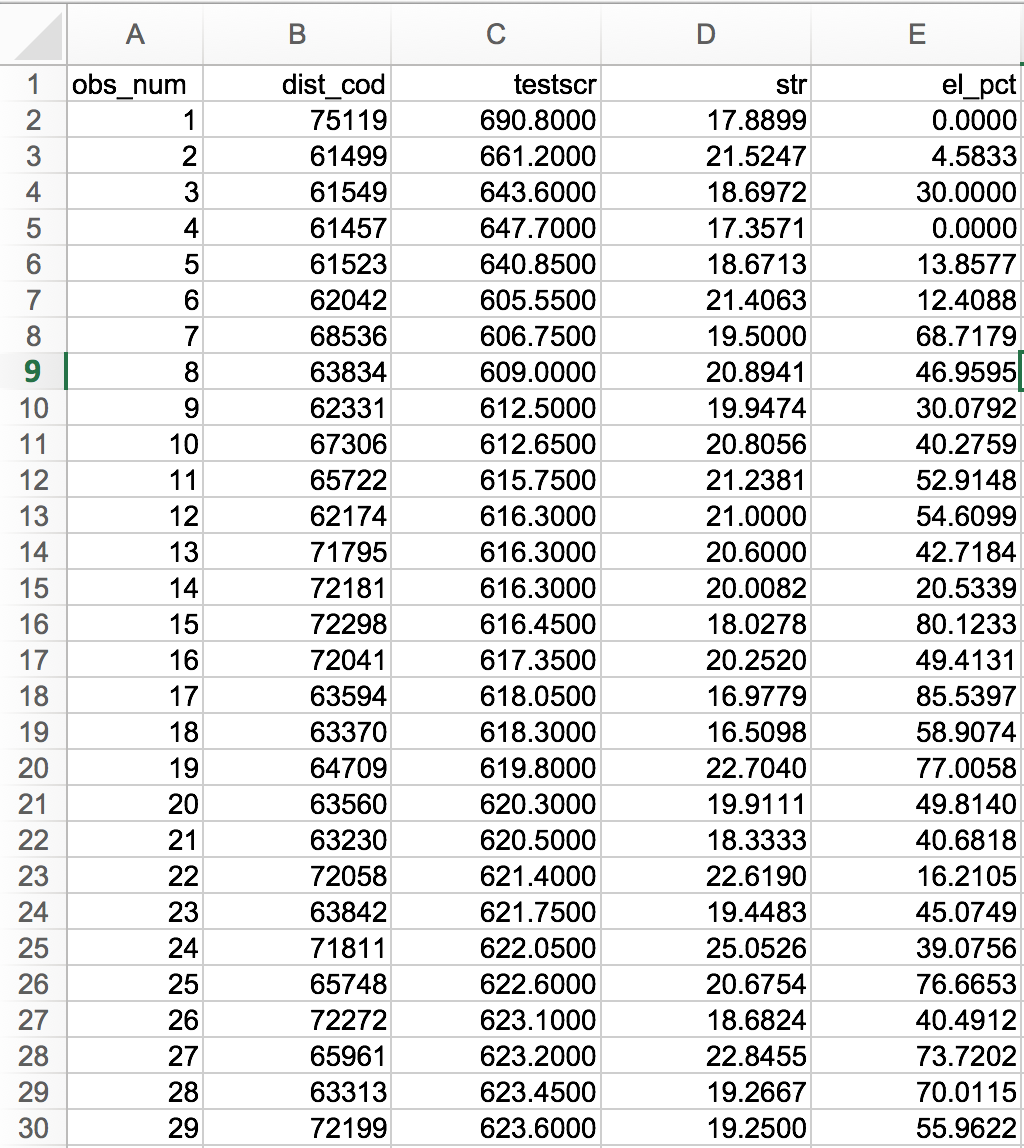
\includegraphics[width=0.6\textwidth,height=0.6\textwidth]{img/data_snapshot.png}
\caption{\label{fig:org1ba8b7d}
The California data set in spreadsheet}
\end{figure}

Each row represents an observation of all variables pertaining to a
school district, and each column represents a variable with all
observations. This format of data display can be concisely denoted
using vectors and a matrix.

Let us first define the following vectors and matrices:
\begin{equation*}
\mathbf{Y} =
\begin{pmatrix}
Y_1 \\
Y_2 \\
\vdots \\
Y_n
\end{pmatrix},\,
\mathbf{X} =
\begin{pmatrix}
1 & X_{11} & \cdots & X_{k1} \\
1 & X_{12} & \cdots & X_{k2} \\
\vdots & \vdots & \ddots & \vdots \\
1 & X_{1n} & \cdots & X_{kn}
\end{pmatrix}
=
\begin{pmatrix}
\mathbi{x}^{\prime}_1 \\
\mathbi{x}^{\prime}_2 \\
\vdots \\
\mathbi{x}^{\prime}_n
\end{pmatrix},\,
\mathbf{u} =
\begin{pmatrix}
u_1 \\
u_2 \\
\vdots \\
u_n
\end{pmatrix},\,
\boldsymbol{\beta} =
\begin{pmatrix}
\beta_0 \\
\beta_1 \\
\vdots \\
\beta_k
\end{pmatrix}
\end{equation*}

\begin{itemize}
\item \(\mathbf{Y}\) is an \(n \times 1\) vector of \(n\) observations on the
dependent variable.
\item \(\mathbf{X}\) is an \(n \times (k+1)\) matrix of \(n\) observations on
\(k + 1\) regressors which include the intercept term as a regressor of
1's.
\item \(\mathbi{x}_i\) is a \((k+1) \times 1\) vector of the i\(^{\text{th}}\)
observation on all \((k+1)\) regressors. Thus,
\(\mathbi{x}^{\prime}_i\) denotes the i\(^{\text{th}}\) row in \(\mathbf{X}\).
\item \(\boldsymbol{\beta}\) is a \((k+1) \times 1\) vector of the \((k+1)\)
regression coefficients.
\item \(\mathbf{u}\) is an \(n \times 1\) vector of the \(n\) error terms.
\end{itemize}

\subsubsection*{Write a multiple regression model with matrix notation}
\label{sec:org13c9179}
\begin{itemize}
\item The multiple regression model for one observation
\label{sec:org1ae6d00}

The multiple regression model in Equation (\ref{eq:multi-regress-1})
for the i\(^{\text{th}}\) observation can be written as
\begin{equation}
\label{eq:multi-regress-mi}
Y_i = \mathbi{x}^{\prime}_i \boldsymbol{\beta} + u_i,\; i = 1, \ldots, n
\end{equation}

\item The multiple regression model for all observations
\label{sec:org870b83d}

Stacking all \(n\) observations in Equation (\ref{eq:multi-regress-mi})
yields the multiple regression model in matrix form:
\begin{equation}
\label{eq:multi-regress-m}
\mathbf{Y} = \mathbf{X} \boldsymbol{\beta} + \mathbf{u}
\end{equation}

\(\mathbf{X}\) can also be written in terms of column vectors as
\[
\mathbf{X} = [\mathbf{X}_0, \mathbf{X}_1, \ldots, \mathbf{X}_k ]
\]
where \(\mathbf{X}_i = [X_{i1}, X_{i2}, \ldots, X_{in}]^{\prime}\) is a
\(n \times 1\) vector of \(n\) observations of the k\(^{\text{th}}\)
regressor. \(\mathbf{X}_0\) is a vector of 1s. That is,
\(\mathbf{X}_0 = [1, 1, \ldots, 1]^{\prime}\). More often, we use
\(\boldsymbol{\iota}\) to denote such a vector of 1s. \footnote{\(\boldsymbol{\iota}\) has the following properties:
(1) \(\boldsymbol{\iota}^{\prime} \mathbf{x} = \sum_{i=1}^n x_i\) for an
\(n \times 1\) vector \(\mathbf{x}\), (2) \(\boldsymbol{\iota}^{\prime}
\boldsymbol{\iota} = n\) and \(\left(\boldsymbol{\iota}^{\prime}
\boldsymbol{\iota} \right)^{-1} = 1/n\), (3)
\(\boldsymbol{\iota}^{\prime} \left(
\boldsymbol{\iota}^{\prime}\boldsymbol{\iota} \right)^{-1} \mathbf{x}
= \bar{x}\), and (4) \(\boldsymbol{\iota}^{\prime} \mathbf{X} \boldsymbol{\iota} =
  \sum_{i=1}^n \sum_{j=1}^n x_{ij}\) for an \(n \times n\) matrix \(\mathbf{X}\).}

Thus, Equation (\ref{eq:multi-regress-m}) can be re-written as
\begin{equation}
\label{eq:multi-regress-m2}
\mathbf{Y} = \beta_0\boldsymbol{\iota} + \beta_1\mathbf{X}_1 + \cdots + \beta_k\mathbf{X}_k + \mathbf{u}
\end{equation}
\end{itemize}


\section{The OLS Estimator in Multiple Regression}
\label{sec:orgb4bf112}

\subsection{The OLS estimator}
\label{sec:org1d21bb0}

\subsubsection*{The minimization problem}
\label{sec:org45208f6}

The idea of the ordinary least squares estimation for a multiple
regression model is exactly the same as for a simple regression
model. The OLS estimators of the multiple regression model are obtained by
minimizing the sum of the squared prediction mistakes.

Let \(\mathbf{b} = [b_0, b_1, \ldots, b_k]^{\prime}\) be some estimators of
\(\boldsymbol{\beta} = [\beta_0, \beta_1, \ldots,
\beta_k]^{\prime}\). The predicted \(Y_i\) can be obtained by
\[ \hat{Y}_i = b_0 + b_1 X_{1i} + \cdots + b_k X_{ki} = \mathbi{x}^{\prime}_i
\mathbf{b},\, i = 1, \ldots, n \]
or in matrix notation
\[ \hat{\mathbf{Y}} = \mathbf{Xb} \]

The prediction mistakes with \(\mathbf{b}\), or called the residuals, are
\[ \hat{u}_i = Y_i - b_0 - b_1 X_{1i} - \cdots - b_k X_{ki} = Y_i -
\mathbi{x}^{\prime}_i \mathbf{b} \]
or in matrix notation, the residual vector is
\[ \hat{\mathbf{u}} = \mathbf{Y} - \mathbf{Xb} \]

Then the sum of the squared prediction mistakes (residuals) is
\begin{align*}
S(\mathbf{b}) & = S(b_0, b_1, \ldots, b_k) = \sum_{i=1}^n (Y_i - b_0 - b_1 X_{1i} - \cdots - b_k X_{ki})^2 \\
& = \sum_{i=1}^n (Y_i - \mathbi{x}^{\prime}_i \mathbf{b})^2 = (\mathbf{Y} -
\mathbf{Xb})^{\prime}(\mathbf{Y}-\mathbf{Xb}) \\
& = \hat{\mathbf{u}}^{\prime} \hat{\mathbf{u}} = \sum_{i=1}^n \hat{u}_i^2
\end{align*}

The OLS estimator is the solution to the following minimization problem:
\begin{equation}
\label{eq:ols-multi-regress}
\operatorname*{min}_{\mathbf{b}}\: S(\mathbf{b}) = \hat{\mathbf{u}}^{\prime} \hat{\mathbf{u}}
\end{equation}

\subsubsection*{The OLS estimator of \(\boldsymbol{\beta}\) as a solution to the minimization problem}
\label{sec:orgc512bf5}

The formula for the OLS estimator is obtained by taking the derivative
of the sum of squared prediction mistakes, \(S(b_0, b_1, \ldots, b_k)\), with respect to each coefficient,
setting these derivatives to zero, and solving for the estimator
\(\hat{\boldsymbol{\beta}}\).

The derivative of \(S(b_0, \ldots, b_k)\) with respect to \(b_j\) is
\begin{gather*}
\label{eq:ols-wrt-bj}
\frac{\partial }{\partial b_j} \sum_{i=1}^n \left(Y_i - b_0 - b_1 X_{1i} - \cdots - b_k X_{ki} \right)^2 = \\
-2 \sum_{i=1}^n X_{ji} \left(Y_i - b_0 - b_1 X_{1i} - \cdots - b_k X_{ki} \right) = 0
\end{gather*}
There are \(k+1\) such equations for \(j=0, \ldots, k\). Solving this
system of equations, we obtain the OLS estimator
\(\hat{\boldsymbol{\beta}} = (\hat{\beta}_0, \ldots, \hat{\beta}_k)^{\prime}\).

Using matrix notation, the formula for the OLS estimator
\(\boldsymbol{\hat{\beta}}\) is
\begin{equation}
\label{eq:betahat-mult}
\boldsymbol{\hat{\beta}} = (\mathbf{X}^{\prime} \mathbf{X})^{-1} \mathbf{X}^{\prime} \mathbf{Y}
\end{equation}

To prove Equation (\ref{eq:betahat-mult}), we need to use some results
of matrix calculus.
\begin{equation}
\label{eq:matrix-calc}
\frac{\partial \mathbf{a}^{\prime} \mathbf{x}}{\partial \mathbf{x}} = \mathbf{a},\; \frac{\partial \mathbf{x}^{\prime} \mathbf{a}}{\partial \mathbf{x}} = \mathbf{a},\; \text{ and } \frac{\partial \mathbf{x}^{\prime} \mathbf{A} \mathbf{x}}{\partial \mathbf{x}} = (\mathbf{A} + \mathbf{A}^{\prime}) \mathbf{x}
\end{equation}
when \(\mathbf{A}\) is symmetric, then \((\partial \mathbf{x}^{\prime} \mathbf{A} \mathbf{x}) / (\partial \mathbf{x}) = 2\mathbf{A} \mathbf{x}\)

\begin{proof}[Proof of Equation (\ref{eq:betahat-mult})]
The sum of squared prediction mistakes is
\begin{equation*}
S(\mathbf{b}) = \hat{\mathbf{u}}^{\prime} \hat{\mathbf{u}} = \mathbf{Y}^{\prime} \mathbf{Y} - \mathbf{b}^{\prime} \mathbf{X}^{\prime} \mathbf{Y} - \mathbf{Y}^{\prime} \mathbf{Xb} - \mathbf{b}^{\prime} \mathbf{X}^{\prime} \mathbf{Xb}
\end{equation*}
The first order conditions for minimizing $S(\mathbf{b})$ with respect to $\mathbf{b}$ is
\begin{equation}
\label{eq:ols-mult-eqs}
-2 \mathbf{X}^{\prime} \mathbf{Y} - 2 \mathbf{X}^{\prime} \mathbf{Xb} = \mathbf{0}
\end{equation}
Then
\begin{equation*}
\mathbf{b} = (\mathbf{X}^{\prime} \mathbf{X})^{-1} \mathbf{X}^{\prime} \mathbf{Y}
\end{equation*}
given that $\mathbf{X}^{\prime} \mathbf{X}$ is invertible.
\end{proof}

Note that Equation (\ref{eq:ols-mult-eqs}) represents a system of
equations with \(k+1\) equations.


\subsection{Example: the OLS estimator of \(\hat{\beta}_1\) in a simple regression model}
\label{sec:org9171e23}

Let take a simple linear regression model as an example. The simple
linear regression model written in matrix notation is
\begin{equation*}
\mathbf{Y} = \beta_0 \boldsymbol{\iota} + \beta_1 \mathbf{X}_1 + \mathbf{u} = \mathbf{X} \boldsymbol{\beta} + \mathbf{u}
\end{equation*}
where

\begin{equation*}
\mathbf{Y} =
\begin{pmatrix}
Y_1 \\
\vdots \\
Y_n
\end{pmatrix},\,
\mathbf{X} =
\begin{pmatrix}
\boldsymbol{\iota} & \mathbf{X}_1
\end{pmatrix}
=
\begin{pmatrix}
1 & X_{11} \\
\vdots & \vdots \\
1 & X_{1n}
\end{pmatrix},\,
\mathbf{u} =
\begin{pmatrix}
u_1 \\
\vdots \\
u_n
\end{pmatrix},\,
\boldsymbol{\beta} =
\begin{pmatrix}
\beta_0 \\
\beta_1 \\
\end{pmatrix}
\end{equation*}

Let's get the components in Equation (\ref{eq:betahat-mult}) step by
step.

First, the most important part is
\(\left(\mathbf{X}^{\prime}\mathbf{X}\right)^{-1}\).

\begin{align*}
\mathbf{X}^{\prime}\mathbf{X} &=
\begin{pmatrix}
\boldsymbol{\iota}^{\prime} \\
\mathbf{X}_1^{\prime}
\end{pmatrix}
\begin{pmatrix}
\boldsymbol{\iota} & \mathbf{X}_1
\end{pmatrix} =
\begin{pmatrix}
1 & \cdots & 1 \\
X_{11} & \cdots & X_{1n}
\end{pmatrix}
\begin{pmatrix}
1 & X_{11} \\
\vdots & \vdots \\
1 & X_{1n}
\end{pmatrix} \\
&=
\begin{pmatrix}
\boldsymbol{\iota}^{\prime} \boldsymbol{\iota} & \boldsymbol{\iota}^{\prime} \mathbf{X}_1 \\
\mathbf{X}_1^{\prime} \boldsymbol{\iota} & \mathbf{X}_1^{\prime} \mathbf{X}_1
\end{pmatrix} =
\begin{pmatrix}
n & \sum_{i=1}^n X_{1i} \\
\sum_{i=1}^n X_{1i} & \sum_{i=1}^n X_{1i}^2
\end{pmatrix}
\end{align*}

Recall that the inverse of a \(2 \times 2\) matrix can be calculated as follows
\begin{equation*}
\begin{pmatrix}
a_{11} & a_{12} \\
a_{21} & a_{22}
\end{pmatrix}^{-1}
=\frac{1}{a_{11}a_{22} - a_{12}a_{21}}
\begin{pmatrix}
a_{22} & -a_{12} \\
-a_{21} & a_{11}
\end{pmatrix}
\end{equation*}

Thus, the inverse of \(\mathbf{X}^{\prime}\mathbf{X}\) is
\begin{equation*}
\left(\mathbf{X}^{\prime}\mathbf{X}\right)^{-1} =
\frac{1}{n \sum_{i=1}^n X_{1i}^2 - (\sum_{i=1}^n X_{1i})^2}
\begin{pmatrix}
\sum_{i=1}^n X_{1i}^2 & - \sum_{i=1}^n X_{1i} \\
-\sum_{i=1}^n X_{1i} & n
\end{pmatrix}
\end{equation*}

Next, we compute \(\mathbf{X}^{\prime} \mathbf{Y}\).
\begin{equation*}
\mathbf{X}^{\prime} \mathbf{Y} =
\begin{pmatrix}
\boldsymbol{\iota}^{\prime} \\
\mathbf{X}_1^{\prime}
\end{pmatrix}
\mathbf{Y} =
\begin{pmatrix}
1 & \cdots & 1 \\
X_{11} & \cdots & X_{1n}
\end{pmatrix}
\begin{pmatrix}
Y_1 \\
\vdots \\
Y_n
\end{pmatrix} =
\begin{pmatrix}
\boldsymbol{\iota}^{\prime} \mathbf{Y} \\
\mathbf{X}_1^{\prime} \mathbf{Y}
\end{pmatrix} =
\begin{pmatrix}
\sum_{i=1}^n Y_i \\
\sum_{i=1}^n X_{1i} Y_i
\end{pmatrix}
\end{equation*}

Finally, we compute \(\boldsymbol{\hat{\beta}} = (\mathbf{X}^{\prime}
\mathbf{X})^{-1} \mathbf{X}^{\prime} \mathbf{Y}\), which is
\begin{align*}
\begin{pmatrix}
\hat{\beta}_0 \\
\hat{\beta}_1
\end{pmatrix} & =
\frac{1}{n \sum_{i=1}^n X_{1i}^2 - (\sum_{i=1}^n X_{1i})^2}
\begin{pmatrix}
\sum_{i=1}^n X_{1i}^2 & - \sum_{i=1}^n X_{1i} \\
-\sum_{i=1}^n X_{1i} & n
\end{pmatrix}
\begin{pmatrix}
\sum_{i=1}^n Y_i \\
\sum_{i=1}^n X_{1i} Y_i
\end{pmatrix} \\
& =
\frac{1}{n \sum_{i=1}^n X_{1i}^2 - (\sum_{i=1}^n X_{1i})^2}
\begin{pmatrix}
\sum_{i=1}^n X_{1i}^2 \sum_{i=1}^n Y_i - \sum_{i=1}^n X_{1i} \sum_{i=1}^n X_{1i}Y_i \\
-\sum_{i=1}^n X_{1i} \sum_{i=1}^n Y_i + n \sum_{i=1}^n X_{1i} Y_i
\end{pmatrix}
\end{align*}

Therefore, \(\hat{\beta}_1\) is the second element of the vector
pare-multiplied by the fraction, that is,
\begin{equation*}
\hat{\beta}_1 = \frac{n \sum_{i=1}^n X_{1i} Y_i - \sum_{i=1}^n X_{1i} \sum_{i=1}^n Y_i}{n \sum_{i=1}^n X_{1i}^2 - (\sum_{i=1}^n X_{1i})^2} = \frac{\sum_{i=1}^n (X_{1i} - \bar{X}_1)(Y_i - \bar{Y})}{\sum_{i=1}^n (X_{1i} - \bar{X}_1)^2}
\end{equation*}

It follows that
\begin{equation*}
\hat{\beta}_0 = \frac{\sum_{i=1}^n X_{1i}^2 \sum_{i=1}^n Y_i - \sum_{i=1}^n X_{1i} \sum_{i=1}^n X_{1i}Y_i}{n \sum_{i=1}^n X_{1i}^2 - (\sum_{i=1}^n X_{1i})^2} = \bar{Y} - \hat{\beta}_1 \bar{X}_1
\end{equation*}


\subsection{Application to Test Scores and the Student-Teacher Ratio}
\label{sec:org78a2779}

Now we can apply the OLS estimation method of multiple regression to
the application of California school districts. Recall that the
estimated simple linear regression model is
\[ \widehat{TestScore} = 698.9 - 2.28 \times STR \]

Since we concern that the estimated coefficient on \emph{STR} may be
overestimated without considering the percentage of English
learners in the districts, we include this new variable in the
multiple regression model to control for the effect of English
learners, yielding a new estimated regression model as
\[ \widehat{TestScore} = 686.0 - 1.10 \times STR - 0.65 \times PctEL
\]
\begin{itemize}
\item The interpretation of the new estimated coefficient on \emph{STR} is,
\textbf{holding the percentage of English learners constant}, a unit
decrease in \emph{STR} is estimated to increase test scores by 1.10
points.
\item We can also interpret the estimated coefficient on \emph{PctEL} as,
holding \emph{STR} constant, one unit decrease in \emph{PctEL} increases test
scores by 0.65 point.
\item The magnitude of the negative effect of \emph{STR} on test scores in the
multiple regression is approximately half as large as when \emph{STR} is
the only regressor, which verifies our concern that we may omit
important variables in the simple linear regression model.
\end{itemize}


\section{Measures of Fit in Multiple Regression}
\label{sec:orgc558526}

\subsection{The Standard errors of the regression (SER)}
\label{sec:orgea3093a}

The standard error
of regression (SER) estimates the standard deviation of the error term
\(\mathbf{u}\). In multiple regression, the SER is
\begin{equation}
\label{eq:ser-m}
SER = s_{\hat{u}},\; \text{ where } s^2_{\hat{u}} = \frac{1}{n-k-1} \sum_{i=1}^n \hat{u}_i^2 =\frac{\mathbf{\hat{u}}^{\prime} \mathbf{\hat{u}}}{n-k-1} = \frac{SSR}{n-k-1}
\end{equation}
Here \(SSR\) is divided by \((n-k-1)\) because there are \((k+1)\)
coefficients to be estimated using \(n\) samples.


\subsection{\(R^2\)}
\label{sec:org29ad69f}

\subsubsection*{The definition of \(R^2\) in multiple regression models}
\label{sec:orgcade614}

Like in the regression model with single regressor, we can define
\(TSS\), \(ESS\), and \(SSR\) in the multiple regression model.

\begin{itemize}
\item \textbf{The total sum of squares (TSS)}: \(TSS = \sum_{i=1}^n (Y_i - \bar{Y})^2\)
\item \textbf{The explained sum of squares (ESS)}: \(ESS = \sum_{i=1}^n (\hat{Y}_i - \bar{Y})^2\)
\item \textbf{The sum of squared residuals (SSR)}: \(SSR = \sum_{i=1}^n \hat{u}_i^2\)
\end{itemize}

Let \(y_i\) be the deviation of \(Y_i\) from its sample mean, that it,
\(y_i = Y_i - \bar{Y},\; i=1,\ldots,n\). In matrix notation, we have
\begin{equation*}
\mathbf{Y} =
\begin{pmatrix}
Y_1 \\
Y_2 \\
\vdots \\
Y_n
\end{pmatrix},\;
\boldsymbol{\iota} =
\begin{pmatrix}
1 \\
1 \\
\vdots \\
1
\end{pmatrix},\;
\mathbf{y} =
\begin{pmatrix}
y_1 \\
y_2 \\
\vdots \\
y_n
\end{pmatrix}
=
\begin{pmatrix}
Y_1 \\
Y_2 \\
\vdots \\
Y_n
\end{pmatrix}
-
\begin{pmatrix}
\bar{Y} \\
\bar{Y} \\
\vdots \\
\bar{Y}
\end{pmatrix}
=
\mathbf{Y} - \bar{Y} \boldsymbol{\iota}
\end{equation*}
Therefore, \(\mathbf{y}\) is the vector of the deviation from the mean of
\(Y_i,\; i=1,\ldots,n\). Similarly, we can define the deviation from the
mean of \(\hat{Y}_i,\, i=1, \ldots, n\) as \(\hat{\mathbf{y}} =
\hat{\mathbf{Y}} - \bar{Y} \boldsymbol{\iota}\). Then we can rewrite
\(TSS, ESS,\, \text{ and } SSR\) as
\[ TSS = \mathbf{y}^{\prime} \mathbf{y},\; ESS =
\hat{\mathbf{y}}^{\prime} \hat{\mathbf{y}},\; \text{ and } SSR =
\hat{\mathbf{u}}^{\prime} \hat{\mathbf{u}} \]

In multiple regression, the relationship that
\[ TSS = ESS + SSR, \text{ or, } \mathbf{y}^{\prime} \mathbf{y} =
\hat{\mathbf{y}}^{\prime} \hat{\mathbf{y}} + \hat{\mathbf{u}}^{\prime}
\hat{\mathbf{u}}\]
still holds so that we can define \(R^2\) as
\begin{equation}
\label{eq:r2-center}
R^2 = \frac{ESS}{TSS} = 1 - \frac{SSR}{TSS}
\end{equation}

\subsubsection*{Limitations of \(R^2\)}
\label{sec:org2cbdb3b}

\begin{enumerate}
\item \(R^2\) is valid only if a regression model is estimated using the OLS
since otherwise it would not be true that \(TSS = ESS + SSR\).

\item \(R^2\) defined in the form of the deviation from the mean is only
valid when a constant term is included in regression. Otherwise,
use the uncentered version of \(R^2\), which is also defined as
\begin{equation}
\label{eq:r2-uncenter}
R^2_u = \frac{EES}{TSS} = 1 - \frac{SSR}{TSS}
\end{equation}
where \(TSS = \sum_{i=1}^n Y_i^2 = \mathbf{Y}^{\prime} \mathbf{Y}\),
\(ESS = \sum_{i=1}^2 \hat{Y}_i^2 = \hat{\mathbf{Y}}^{\prime}
   \hat{\mathbf{Y}}\), and \(SSR = \sum_{i=1}^n \hat{u}_i^2 =
   \hat{\mathbf{u}}^{\prime} \hat{\mathbf{u}}\), using the uncentered
variables.  Note that in a regression without a constant term, the
equality \(TSS = ESS + SSR\) is still true.

\item Most importantly, \(R^2\) increases whenever an additional regressor
is included in a multiple regression model, unless the estimated
coefficient on the added regressor is exactly zero. 

Consider two regression models
\begin{align}
\mathbf{Y} &= \beta_0 + \beta_1 \mathbf{X}_1 + \mathbf{u}
\label{eq:ex-eq-1} \\
\mathbf{Y} &= \beta_0 + \beta_1 \mathbf{X}_1 + \beta_2 \mathbf{X}_2 + \mathbf{u} \label{eq:ex-eq-2}
\end{align}

Since both models use the same \(\mathbf{Y}\), \(TSS\) must be the
same. If the OLS estimator \(\hat{\beta}_2\) does not equal 0, then
\(SSR\) in Equation (\ref{eq:ex-eq-1}) is always larger than that of
Equation (\ref{eq:ex-eq-2})  since the former \(SSR\) is minimized
with respect to \(\beta_0, \beta_1\) and with the constraint of
\(\beta_2 = 0\) and the latter is minimized without the constraint
over \(\beta_2\).
\end{enumerate}


\subsection{The adjusted \(R^2\)}
\label{sec:orgc972d21}

\subsubsection*{The definition of the adjusted \(R^2\)}
\label{sec:orgecd1ff3}

The adjusted \(R^2\) is, or \(\bar{R}^2\), is a modified version of
\(R^2\) in Equation (\ref{eq:r2-center}). \(\bar{R}^2\) improves \(R^2\) in the sense that it does not
necessarily increase when a new regressor is added. 

\(\bar{R}^2\) is
defined as
\begin{equation}
\label{eq:adj-r2}
\bar{R}^2 = 1 - \frac{SSR / (n-k-1)}{TSS / (n-1)} = 1 - \frac{n-1}{n-k-1}\frac{SSR}{TSS} = 1 - \frac{s^2_u}{s^2_Y}
\end{equation}

\begin{itemize}
\item The adjustment is made by dividing \(SSR\) and \(TSS\) by their
corresponding degrees of freedom, which is \(n-k-1\) and \(n-1\),
respectively.
\item \(s^2_u\) is the sample variance of the OLS residuals, which is given
in Equation (\ref{eq:ser-m}); \(s^2_Y\) is the sample variance of \(Y\).
\item The definition of \(\bar{R}^2\) in Equation (\ref{eq:adj-r2}) is
valid only when a constant term is included in the regression
model.
\item Since \(\frac{n-1}{n-k-1} > 1\), then it is always true that
the \(\bar{R}^2 < R^2\).
\item On one hand, \(k \uparrow\, \Rightarrow\, \frac{SSR}{TSS} \downarrow\). On
the other hand, \(k \uparrow\, \Rightarrow \frac{n-1}{n-k-1}
  \uparrow\). Whether \(\bar{R}^2\) increases or decreases depends on
which of these effects is stronger.
\item The \(\bar{R}^2\) can be negative. This happens when the regressors,
taken together, reduce the sum of squared residuals by such a small
amount that his reduction fails to offset the factor \(\frac{n-1}{n-k-1}\).
\end{itemize}

\subsubsection*{The usefulness of \(R^{2}\) and \(\bar{R}^2\)}
\label{sec:org8b5847e}

\begin{itemize}
\item Both \(R^2\) and \(\bar{R}^2\) are valid when the regression model is
estimated by the OLS estimators. \(R^2\) or \(\bar{R}^2\) computed with the
estimators other than the OLS estimators is usually called \emph{pseudo}
\(R^2\).

\item Their importance as measures of fit cannot be overstated. We cannot heavily
reply on \(R^{2}\) or \(\bar{R}^2\) to judge whether some regressors should
be included in the model or not.
\end{itemize}


\section{The Frisch-Waugh-Lovell Theorem}
\label{sec:orgb996807}

\subsection{The grouped regressors}
\label{sec:org4293f71}

Consider a multiple regression model
\begin{equation}
\label{eq:fwl-eq}
Y_i = \underbrace{\beta_0 + \beta_1 X_{1i} +
\cdots + \beta_{k1} X_{k1,i}}_{\text{k1+1 regressors}} + \underbrace{
\beta_{k1+1} X_{k1+1,i} + \cdots \beta_k X_k}_{\text{k2 regressors}} + u_i
\end{equation}

In Equation \eqref{eq:fwl-eq}, among k regressors, \(X_1, \ldots, X_k\),
we collect \(k1\) regressors and an intercept into a group and the rest
\(k2 = k - k1\) regressors into a second group. In matrix notation,
we write
\begin{equation}
\label{eq:mult-reg-2g}
\mathbf{Y} = \mathbf{X}_1\boldsymbol{\beta}_1 + \mathbf{X}_2 \boldsymbol{\beta}_2 + \mathbf{u}
\end{equation}
where \(\mathbf{X}_1\) is an \(n \times (k1+1)\) matrix composed of the
intercept and the first \(k1+1\) regressors in Equation \eqref{eq:fwl-eq},
and \(\mathbf{X}_2\) is an \(n \times k2\) matrix composed of the rest
\(k_2\) regressors. \(\boldsymbol{\beta}_1 = (\beta_0, \beta_1, \ldots,
\beta_{k1})^{\prime}\) and \(\boldsymbol{\beta}_2 = (\beta_{k1+1},
\ldots, \beta_k)^{\prime}\). 


\subsection{Two estimation strategies}
\label{sec:org3f45358}

Suppose that we are interested in \(\boldsymbol{\beta}_2\) but not much
in \(\boldsymbol{\beta}_1\) in Equation \eqref{eq:mult-reg-2g}. How can we
estimate \(\boldsymbol{\beta}_2\)?

\subsubsection*{The first strategy: the standard OLS estimation}
\label{sec:org0e943cd}

We can obtain the OLS estimation of \(\boldsymbol{\beta}_2\) with
Equation \eqref{eq:betahat-mult}, i.e., \(\hat{\boldsymbol{\beta}} =
(\mathbf{X}^{\prime} \mathbf{X})^{-1} \mathbf{X}^{\prime}
\mathbf{Y}\). \(\hat{\boldsymbol{\beta}}_2\) is a vector consisting of
the last \(k2\) elements in \(\hat{\boldsymbol{\beta}}\). 

In matrix notation, we can get \(\hat{\boldsymbol{\beta}}_2\) from the
following equation
\begin{equation*}
\begin{pmatrix}
\hat{\boldsymbol{\beta}}_1 \\
\hat{\boldsymbol{\beta}}_2 
\end{pmatrix} =
\begin{pmatrix}
\mathbf{X}_1^{\prime} \mathbf{X}_1 & \mathbf{X}_1^{\prime} \mathbf{X}_2 \\
\mathbf{X}_2^{\prime} \mathbf{X}_1 & \mathbf{X}_2^{\prime} \mathbf{X}_2
\end{pmatrix}^{-1}
\begin{pmatrix}
\mathbf{X}_1^{\prime} \mathbf{Y} \\
\mathbf{X}_2^{\prime} \mathbf{Y}
\end{pmatrix}
\end{equation*}

\subsubsection*{The second strategy: the step OLS estimation}
\label{sec:orgc7b4fbc}

Alternatively, we can perform the following steps to estimate
\(\boldsymbol{\beta}_2\):
\begin{enumerate}
\item Regress each regressor in \(\mathbf{X}_2\) on all regressors in
\(\mathbf{X}_1\), including the intercept, and get the residuals from
this regression, denoted as \(\widetilde{\mathbf{X}}_2\).

That is, for each regressor \(\mathbf{X}_i\) in \(\mathbf{X}_2\),
\(i=k1+1, \ldots, k\), we estimate a multiple regression, 
\[
   \mathbf{X}_i = \gamma_0 + \gamma_1 \mathbf{X}_1 + \cdots +
   \gamma_{k1} \mathbf{X}_{k1} + v \] 
The residuals from this regression is 
\[ \widetilde{\mathbf{X}}_i = X_i - \hat{\gamma}_0 -
   \hat{\gamma}_1 \mathbf{X}_1 - \cdots - \hat{\gamma}_{k1}
   \mathbf{X}_{k1} \] 
As such, we can get an \(n \times k2\) matrix
composed of all the residuals \(\widetilde{\mathbf{X}}_2 =
   (\widetilde{\mathbf{X}}_{k1+1} \cdots \widetilde{\mathbf{X}}_k)\).

\item Regress \(\mathbf{Y}\) on all regressors in \(\mathbf{X}_1\), denoting
the residuals from this regression as \(\widetilde{\mathbf{Y}}\).

\item Regress \(\widetilde{\mathbf{Y}}\) on \(\widetilde{\mathbf{X}}_2\), and
obtain the estimates of \(\boldsymbol{\beta}_2\) as
\(\boldsymbol{\beta}_2=(\widetilde{\mathbf{X}}_2^{\prime} \widetilde{\mathbf{X}}_2)^{-1}
   \widetilde{\mathbf{X}}_2^{\prime} \widetilde{\mathbf{Y}}\).
\end{enumerate}


\subsection{The Frisch-Waugh-Lovell Theorem}
\label{sec:org6edb9ea}

The Frisch-Waugh-Lovell (FWL) Theorem states that
\begin{enumerate}
\item the OLS estimates of \(\boldsymbol{\beta}_2\) using the second strategy
and that from the first strategy are numerically identical.
\item the residuals from the regression of \(\widetilde{\mathbf{Y}}\) on
\(\widetilde{\mathbf{X}}_2\) and the residuals from Equation
(\ref{eq:mult-reg-2g}) are numerically identical.
\end{enumerate}

The proof of the FWL theorem is beyond the scope of this
proof. Interested students may refer to Exercise 18.7.
Understanding the meaning of this theorem is much more important than
understanding the proof.

The FWL theorem provides a mathematical statement of how the multiple
regression coefficients in \(\hat{\boldsymbol{\beta}}_2\) capture the
effects of \(\mathbf{X}_2\) on \(\mathbf{Y}\), controlling for other
\(\mathbf{X}\).

\begin{itemize}
\item Step 1 purges the effects of the regressors in \(\mathbf{X}_1\) on the
regressors in \(\mathbf{X}_2\)
\item Step 2 purges the effects of the regressors in \(\mathbf{X}_1\) on
\(\mathbf{Y}\).
\item Step 3 estimates the effect of the regressors in \(\mathbf{X}_2\) on
\(\mathbf{Y}\) using the parts in \(\mathbf{X}_2\) and
\(\mathbf{Y}\) that have excluded the effects of \(\mathbf{X}_1\).
\end{itemize}

\subsection{An example of the FWL theorem}
\label{sec:org3c6fc1c}
Consider a regression model with single regressor
\[ Y_i = \beta_0 +
\beta_1 X_i + u_i,\; i=1, \ldots, n
\]

Following the estimation strategy in the FWL theorem, we can carry out
the following regressions,
\begin{enumerate}
\item Regress \(Y_i\) on 1. That is, estimate the model
\[ Y_i = \alpha + e_i \]
Then, the OLS estimator of \(\alpha\) is
\(\bar{Y}\) and the residuals is \(y_i = Y_i - \bar{Y}\)
\item Similarly, regress \(X_{i}\) on 1. Then
the residuals from this regression is \(x_{i} = X_{i} -
   \bar{X}\).
\item Regress \(y_i\) on \(x_{i}\) without intercept. That is,
estimate the model
\[ y_i = \beta_1 x_{i} + v_i \]
\item We can obtain \(\hat{\beta_1}\) directly by applying the formula in
Equation (\ref{eq:betahat-mult}). That is 
\[ \hat{\beta}_1 = (\mathbf{x}_1^{\prime} \mathbf{x}_1)^{-1}
   \mathbf{x}_1^{\prime} \mathbf{y} = \frac{\sum_i x_{1i} y_i}{\sum_i
   x_{1i}^2} = \frac{\sum_i (X_i-\bar{X})(Y_i-\bar{Y})}{\sum_i(X_i-\bar{X})^2} \] 
which is exactly the same as the OLS estimator of \(\beta_1\) in \(Y_i
   = \beta_0 + \beta_1 X_i + u_i\).
\end{enumerate}


\section{The Least Squares Assumptions in Multiple Regression}
\label{sec:org4624bd6}

We introduce four least squares assumptions for a multiple regression
model. The first three assumptions are the same as those in the
simple regression model with just minor modifications to suit multiple
regressors. The fourth assumption is a new one. 

\begin{description}
\item[{Assumption \#1}] \(E(u_i | \mathbi{x}_i) = 0\). The conditional mean
of \(u_i\) given \(X_{1i}, X_{2i}, \ldots, X_{ki}\) has
mean of zero. This is the key assumption to assure
that the OLS estimators are unbiased.

\item[{Assumption \#2}] \((Y_i, \mathbi{x}_i^{\prime}),\; i=1, \ldots, n\), are
i.i.d. This assumption holds automatically if the
data are collected by simple random sampling.

\item[{Assumption \#3}] Large outliers are unlikely, i.e.,, \(0 <
                   E(\mathbf{X}^4) < \infty\) and \(0 < E(\mathbf{Y}^4)
                   < \infty\). That is, the dependent variables and
regressors have finite kurtosis.
\item[{Assumption \#4}] No \textbf{perfect multicollinearity}. The regressors are
said to exhibit perfect multicollinearity if one of
the regressor is a perfect linear function of the
other regressors.
\end{description}
\end{document}